\capitolo{Controllo del Moto in presenza di Gioco}
Il gioco è caratterizzato da una variazione dell'inerzia equivalente legata a cambio di segno di \(T_2\) (questo non si verifica in ogni situazione, vedi \ref{giocoViti}. 
Motore e carico possono essere accoppiati per fianco destro o sinistro perciò \(J_{eq} = J_m + \tau^2 J_c\); motore e carico possono essere disaccoppiati \(J_{eq} = J_m\).

\sezione{Problema del gioco}
Il problema legato alla variazione di inerzia è il seguente:
\[
\begin{cases}
    \text{Accoppiati: } J_{eq} = J_m (1+\rho) \ \rightarrow \ \omega_{bv}^{min} \simeq \frac{K_{pv}K_T}{J_m(1+\rho)} \\
    \text{Disaccoppiati: } J_{eq} = J_m \ \rightarrow \ \omega_{bv}^{max} \simeq \frac{K_{pv} K_T}{J_m}
\end{cases}
\]
Ossia passando da carico e motore accoppiati a disaccoppiati, per \(K_{pv}\) costante, la banda passante varia di un fattore \(1+\rho\), l'aumento di banda passante è associato a avvicinamento a \(\omega_I,\omega_{tv}\), che potrebbe portare a calo di margine di fase, e instabilità.

Il gioco è caratterizzato da passaggio imprevedibile da motore carico accoppiati e disaccoppiati, e il cambio tende ad autoalimentarsi, si instaura un ciclo limite di oscillazione non armonica permanente.
Questo problema affligge controllo colocato e non colocato.

\paragrafo{Guadagno di velocità:}
Per limitare gli effetti legati al gioco occorre fare \textbf{riduzione} di \(\mathbf{K_{pv}}\), che va dimensionato in modo da ottenere \(\omega_{bv}^{max} < \omega_{bv}^{lim}\) o comunque tale da garantire un certo margine di fase\footnote{La scelta del margine di fase non dovrebbe essere eccessivamente conservativa, \(m_\phi = 20^\circ\), serve per evitare l'autoalimentazione, dovrebbe servire un numero ridotto di volte per ciclo.} anche per c-m disaccoppiati.

\sottosezione{Rapporto di inerzia}
Il problema del gioco viene semplificato quando viene effettuata la \textbf{riduzione del rapporto di inerzia}, perché porta ad una minore differenza di inerzia tra c-m disaccoppiati/accoppiati, quindi ad avere bande passanti e margini di fase simili.
Tuttavia la scelta di \(\rho\) non dovrebbe portare a utilizzo di riduttori con alto rapporto di trasmissione e gioco elevato.

\begin{figure}[h]
    \centering
    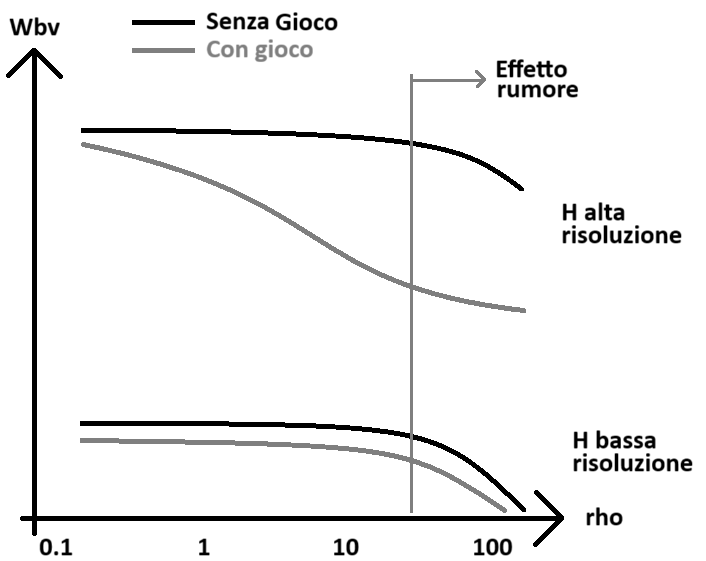
\includegraphics[width=0.45\textwidth]{Immagini/gioco_banda_passante_rho.png}
    \caption{Effetto del gioco: \(\omega_{bv}(\rho)\)}
\end{figure}

\paragrafo{Effetto del rumore:}
Per \(\rho \rightarrow 0\) il gioco è poco rilevante, perché il motore non vede il carico. Le curve calano per \(\rho\) elevati perché portano ad aumentare il \(K_{pv}\) associato, che è quello che fa aumentare gli effetti del rumore. Tuttavia \textbf{non c'è una relazione diretta tra \(\rho\) e aumento del rumore, la causa è l'inerzia totale \(J\), infatti, il calcolo del guadagno per l'anello di posizione è \(K_{pv} = \frac{J \omega_{bv}^{des}}{K_T}\)}, dove facilmente ci si rende conto di questa relazione. Abbassare \(\rho\) aumentando l'inerzia potrebbe peggiorare gli effetti del rumore.

\paragrafo{Rapporto di trasmissione ottimo:}
Riprendendo il rapporto di trasmissione ottimo come visto in \ref{tau_ottimo}, si ottiene, utilizzando una logica diversa, un valore che funziona bene anche per il controllo, dato che porta ad avere \(\rho\) ridotto \footnote{Il motivo non è trasparente, ma intuitivamente la soluzione migliore è quella in cui il motore non ha carico sia in termini meccanici sia in termini di controllo.}.

\sottosezione{Acceleration Feedback}

\import{Immagini/}{acceleration_feedback}

Acceleration Feedback è una tecnica che consiste nel retroazionare l'accelerazione e portarla al motore come corrente, così facendo la relazione tra accelerazione e corrente diventa \(\frac{s^2\theta}{i} = \frac{K_T}{J + K_TK_A}\), ossia viene aumentata virtualmente l'inerzia lato motore di una quantità \(K_TK_A\), da cui si ottiene un rapporto di inerzia virtuale minore, quindi meno sensibile al gioco, \(\rho^\text{virtuale}=\frac{\tau^2 J_c}{J_m + K_TK_A}\).

Tuttavia la misura di accelerazione non è possibile. L'accelerazione può essere stimata a partire dalla misura di posizione utilizzando una doppia derivata e opportuno filtro (il filtro è fondamentale perché la derivata va a amplificare il rumore) oppure utilizzando stimatori complessi (Kalman). In entrambi i casi occorre una misura della posizione molto precisa, inoltre i risultati comunque non sono particolarmente efficaci.\label{misura_acc}

\sottosezione{Load Observer}

\begin{figure}[h]
    \centering
    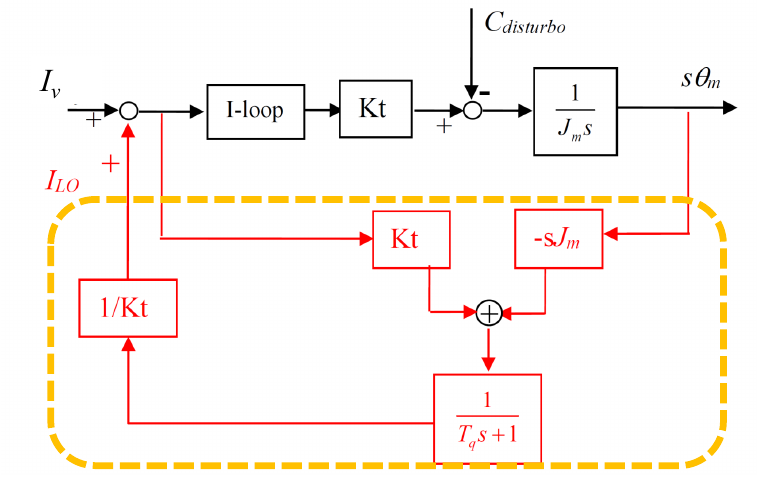
\includegraphics[width=0.5\textwidth]{Immagini/load_observer.png}
    \caption{Load observer, schema implementativo}
\end{figure}

Load Observer è una tecnica che considera il sistema ideale composto dal solo motore, mentre le non idealità vengono consensate in un contributo di coppia di disturbo (gioco e elasticità della trasmissione e attrito).
Se questo contributo di disturbo fosse determinabile, potrebbe essere cancellato (in feedback o eventualmente in feedforward), il sistema ottenuto sarebbe quello ideale solo motore, il carico non viene visto.

Non vedere il carico è il maggior difetto, rimanendo in catena aperta è fondamentale effettuare una opportuna scelta della legge di moto.
Tuttavia significa anche che \(\rho_\text{virtuale} \rightarrow 0\), quindi non c'è sensibilità a gioco, risonanza e antirisonanza virtuali si elidono quindi non c'è sensibilità all'elasticità.

Anche in questo caso è fondamentale la misura di accelerazione, che però ha tutta una serie di problematiche (vedi \ref{misura_acc}).

\paragrafo{Stima della corrente:}
In ingresso al motore viene aggiunta una corrente \(i_{LO}\) tale da generare una coppia uguale e opposta alla coppia di disturbo, in modo si elidano.
\[\begin{cases}
    C_m = K_T i \\
    C_m = J_m \AccAng_m + C_\text{disturbo}
\end{cases} \ \rightarrow \ C_\text{disturbo} = C_m - J_m \AccAng_m = K_T i - J_m \AccAng_m \rightarrow i_{LO} = \frac{K_T i - J_m \AccAng_m}{K_T} \]  

\sottosezione{Esercizio di controllo di un sistema con gioco}
Dati \(J_m=0.001 kgm2, \ K_T=1 Nm/A, \ \rho = 9, \) \( \ \omega_i = 5 kHz, \ \omega_{tv}=700 Hz, \) \( \, \text{Frequenza di campionamento \allowbreak dell’anello di velocità} = 8 kHz\).
Si voglia progettare un controllo tale per cui quando il carico sia disaccoppiato venga garantito un \(m_\phi \simeq 30^\circ\) e che garantisca un margine di fase migliore quando accoppiato.

In condizione di disaccoppiamento deve valere\footnote{Notare che l'inerzia è solo del motore quando carico disaccoppiato.} \(\omega_{bv}^\text{dis} = \omega_a^\text{dis} \simeq \frac{K_{pv}K_T}{J_m}\).

In generale gli aumenti di inerzia causano calo di margine di fase perché provocano uno spostamento della pulsazione di attraversamento che si avvicina all'integrale. Perciò il PI va progettato per carico accoppiato (da carico disaccoppiato ad accoppiato l'inerzia aumenta, inoltre è anche la condizione di lavoro desiderata): \(\frac{1}{T_{iv}} \simeq \frac{\omega_{bv}^\text{acc}}{4\xi^2}\) con \(\omega_{bv}^\text{acc} = \omega_{a}^\text{acc} \simeq \frac{K_{pv}K_T}{J} = \frac{K_{pv}K_T}{J_m (1+\rho)}\).

Nel caso disaccoppiato \(m_\phi^\text{dis} = \pi - \frac{\pi}{2} + \atan{\omega_a^\text{dis} T_{iv}} - \atan{\omega_a^\text{dis} \frac{J}{f}} - \atan{\frac{\omega_a^\text{dis}}{\omega_{tv}}} - \atan{\frac{\omega_a^\text{dis}}{\omega_I}} - \atan{\omega_a^\text{dis} \frac{T_c}{2}} \), considerando un attrito trascurabile, e raccoglieno i termini di trasduttore e anello di corrente in un periodo equivalente \(m_\phi^\text{dis} \simeq \atan{\omega_a^\text{dis} T_{iv}} - \atan{\omega_a^\text{dis} T_{eq}} \). Sostituendo la formula per la sintesi del PI, considerando \(\frac{\omega_a^\text{dis}}{\omega_a^\text{acc}} \simeq 1+\rho\) e in fine sostituendo \(\omega_a^\text{dis}\) nella seconda arcotangente si ottiene: \(m_\phi = \atan{(1+\rho) 4 \xi^2} - \atan{\frac{K_{pv}K_T}{J_m} T_{eq}} \geqslant m_\phi^\text{dis, minima}\).

Da questa espressione è possibile ricavare il guadagno massimo per l'anello di velocità, con \(\xi=1\): \[K_{pv} \leqslant \tan{\left\{\omega_\phi^\text{dis, min} - \atan{4(1+\rho)} \right\}}\frac{J_m}{K_T T_{eq}} \].

Infine è possibile determinare il polo del PI del controllo di velocità \(\frac{1}{T_{iv}} \simeq \frac{\omega_a^\text{acc}}{4\xi^2} \simeq \frac{K_{pv}K_T}{J} \frac{1}{4\xi^2} \).

\sezione{Autotuning}
Con Autotuning si intendono le tecniche di sintonizzazione automatica del controllo a partire da misure sperimentali.
Step:
\begin{enumerate}
    \item Misura di \(L_v(j\omega)\), utilizzata per cercare \(K_{pv}\) che soddisfi \(m_\phi\) e \(m_a\) desiderati o minimi
    \item Calcolo dell'integrale \(\frac{1}{T_{iv}}\) (noi l'abbiamo visto con metodi empirici)
    \item Misura di \(W_v(j\omega)\)
    \item Verifica dell'utente che potrebbe utilizzare dei filtri per cercare eventualmente di migliorare quanto ottenuto
    \item Misura di \(L_p(j\omega)\), utilizzata per sintonizzare \(K_{pp}\)
    \item Misura di \(W_p(j\omega)\)
\end{enumerate}

Occorre prestare attenzione che l'autotuning si basa sulle misure, questo significa che occorre prestare attenzione a una serie di aspetti: scelta di un opportuno numero di misure, encoder sufficientemente risoluto, applicazione di eccitazione di giusta intensità e durata, e come questi devono essere adattati considerando la presenza di gioco.

Attenzione che un controllo ottenuto per autotuning non viene migliorato utilizzando filtri in caso di sistema rigido o con risonanza in bassa frequenza, a meno che non vi siano modi di vibrare di media o alta frequenza che causano problemi in bassa frequenza, in quel caso potrebbero essere utilizzati dei filtri notch (quando i modi di vibrare sono pochi) o dei filtri passa basso.